\documentclass{standalone}
\usepackage{flowchart}
\usepackage{tikz}
\usepackage{amssymb}

\begin{document}
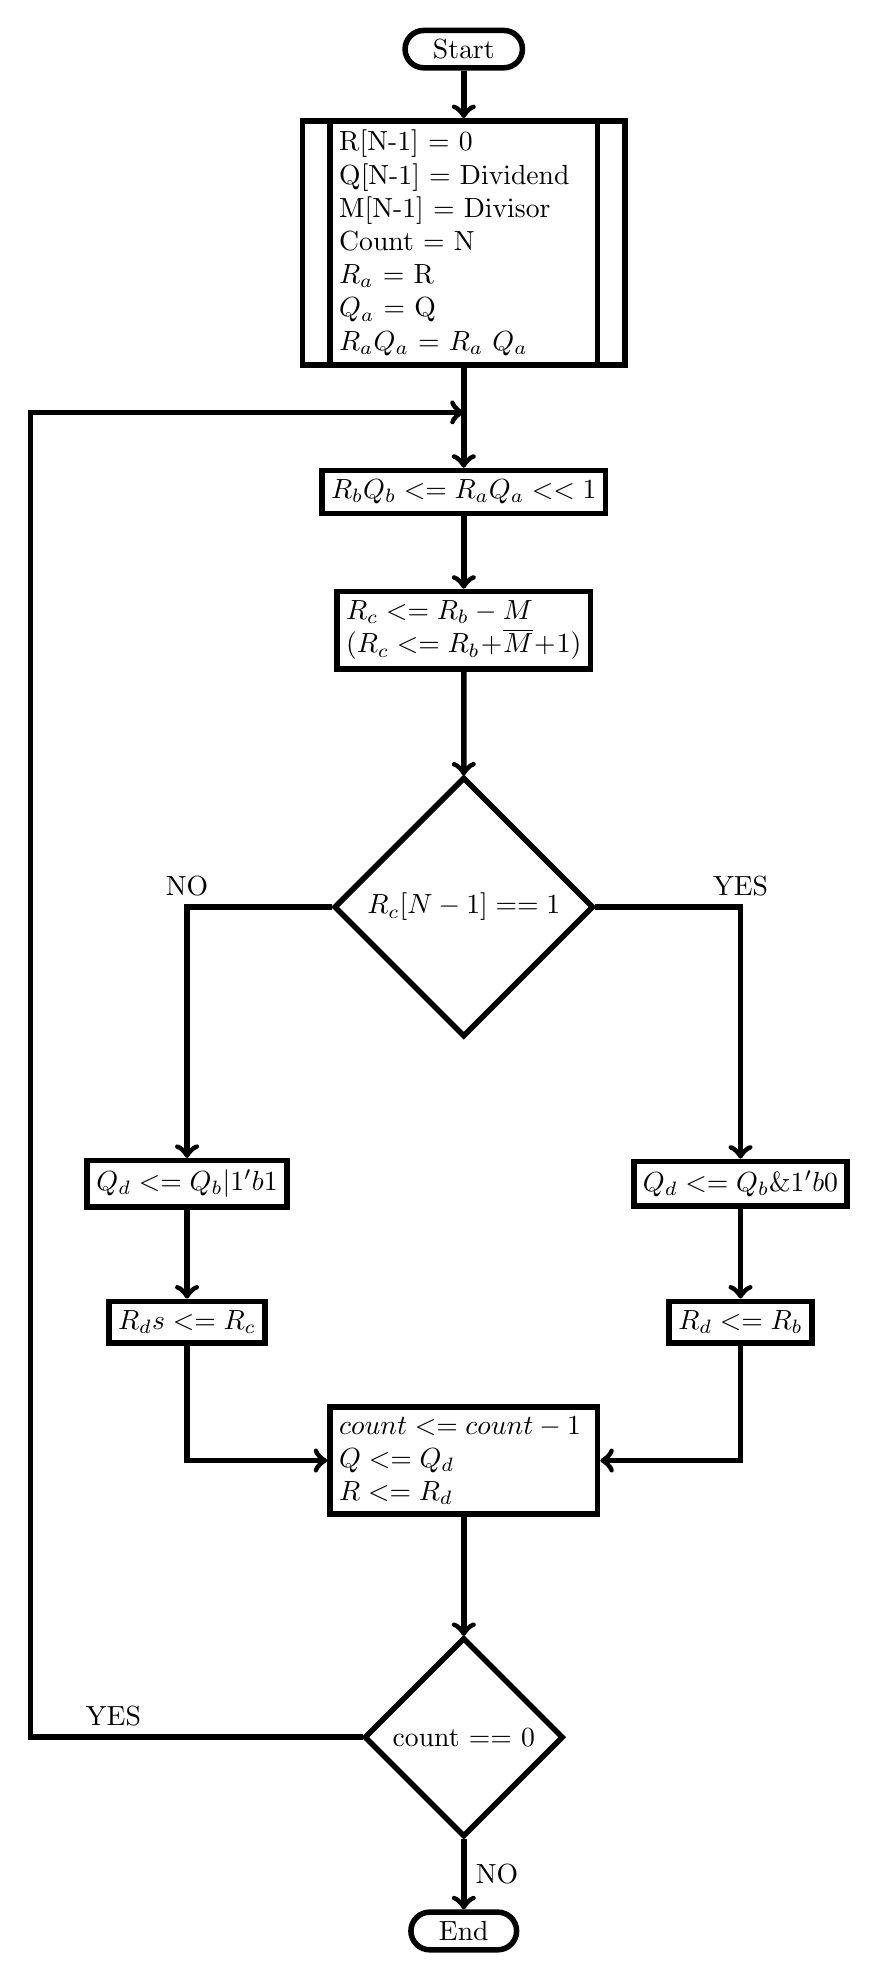
\begin{tikzpicture}[line width=0.2em]
    \node[draw, terminal] (st) at (0,0) {Start};

    \node[draw, predproc, text width=9em] (ini) at ([yshift=-7em]st) {R[N-1] = 0\\Q[N-1] = Dividend\\M[N-1] = Divisor\\Count = N\\ $R_a$ = R\\ $Q_a$ = Q\\ $R_aQ_a$ = {$R_a$ $Q_a$}};


    \node[draw, process] (comb) at ([yshift=-9em]ini) {$R_bQ_b <= R_aQ_a << 1$};


    \node[draw, process, text width=8.5em] (sub) at ([yshift=-5em]comb) {$R_c <= R_b - M$\\ ($R_c <= R_b + \overline{M} + 1$)};


    \node[draw, decision] (dec1) at ([yshift=-10em]sub) {$R_c[N-1] == 1$};

    \node[draw, process] (yes1) at ([xshift=10em, yshift=-10em]dec1) {$Q_d <=  Q_b \& 1'b0$};
    \node[draw, process] (no1) at ([xshift=-10em, yshift=-10em]dec1) {$Q_d <=  Q_b | 1'b1$};

    \node[draw, process] (yes2) at ([xshift=0em, yshift=-5em]yes1) {$R_d <= R_b$};
    \node[draw, process] (no2) at ([xshift=0em, yshift=-5em]no1) {$R_ds <= R_c$};



    \node[draw, process, text width=9em] (counDec) at ([xshift=0em, yshift=-20em]dec1) {$count <= count - 1$\\ $Q <= Q_d$\\ $R <= R_d$};


    \node[draw, decision] (dec2) at ([yshift=-10em]counDec) {count == 0};

    \node[draw, terminal] (ed) at ([yshift=-7em]dec2) {End};

    \draw[->] (st) -- (ini);
    \draw[->] (ini) -- (comb);
    \draw[->] (comb) -- (sub);
    \draw[->] (sub) -- (dec1);

    \draw[->] (dec1.east) -| (yes1.north) node[above, pos=0.5] {YES};
    \draw[->] (dec1.west) -| (no1.north) node[above, pos=0.5] {NO};

    \draw[->] (yes1) -- (yes2);
    \draw[->] (no1) -- (no2);

    \draw[->] (yes2.south) |- (counDec.east);
    \draw[->] (no2.south) |- (counDec.west);

    \draw[->] (counDec.south) -- (dec2.north);

    \draw[->] (dec2.south) -- (ed.north) node[right, pos=0.5] {NO};

    \draw[->] (dec2.west) -- ([xshift=-12em]dec2.west) |- ([yshift=2em]comb.north) node[xshift=3em,above, pos=0] {YES};

\end{tikzpicture}
\end{document}